\frontmatter
\thispagestyle{empty}
\begin{tikzpicture}[remember picture,overlay]
  \def\pw{\paperwidth}\def\ph{\paperheight}
  % teal title band
  \shade[top color=khteal!80!black,bottom color=khteal] (current page.north west) rectangle ($(current page.north east)+(0,-0.365*\paperheight)$);
  \node[text=white,font=\sfb\fontsize{58}{60}\selectfont,inner sep=0] at ($(current page.north)+(0,-0.082*\paperheight)$) {\scalebox{0.74}[1]{PORE-SCALE}};
  \node[text=white,font=\sfb\fontsize{84}{86}\selectfont,inner sep=0] at ($(current page.north)+(0,-0.205*\paperheight)$) {\scalebox{0.70}[1]{DYNAMICS}};
  % authors on a white-to-teal wash
  \shade[left color=white,right color=khteal!25,shading angle=0] ($(current page.north west)+(0,-0.365*\paperheight)$) rectangle ($(current page.north east)+(0,-0.455*\paperheight)$);
  \node[text=khink,font=\sfb\fontsize{15}{18}\selectfont,align=center,inner sep=0] at ($(current page.north)+(0,-0.403*\paperheight)$) {NAZIRU HALILU};
  \node[text=khink,font=\sffamily\fontsize{10}{12}\selectfont,align=center,inner sep=0] at ($(current page.north)+(0,-0.432*\paperheight)$) {Soil water, irrigation and evaporation control};
  % collage
  \node[anchor=north west,inner sep=0] at ($(current page.north west)+(0,-0.455*\paperheight)$) {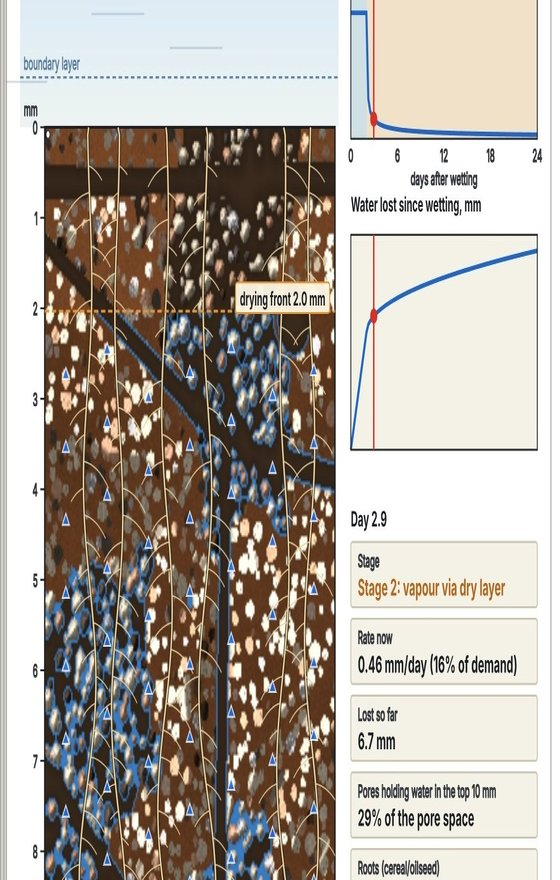
\includegraphics[width=0.33\paperwidth,height=0.37\paperheight]{fig/cv1.jpg}};
  \node[anchor=north east,inner sep=0] at ($(current page.north east)+(0,-0.455*\paperheight)$) {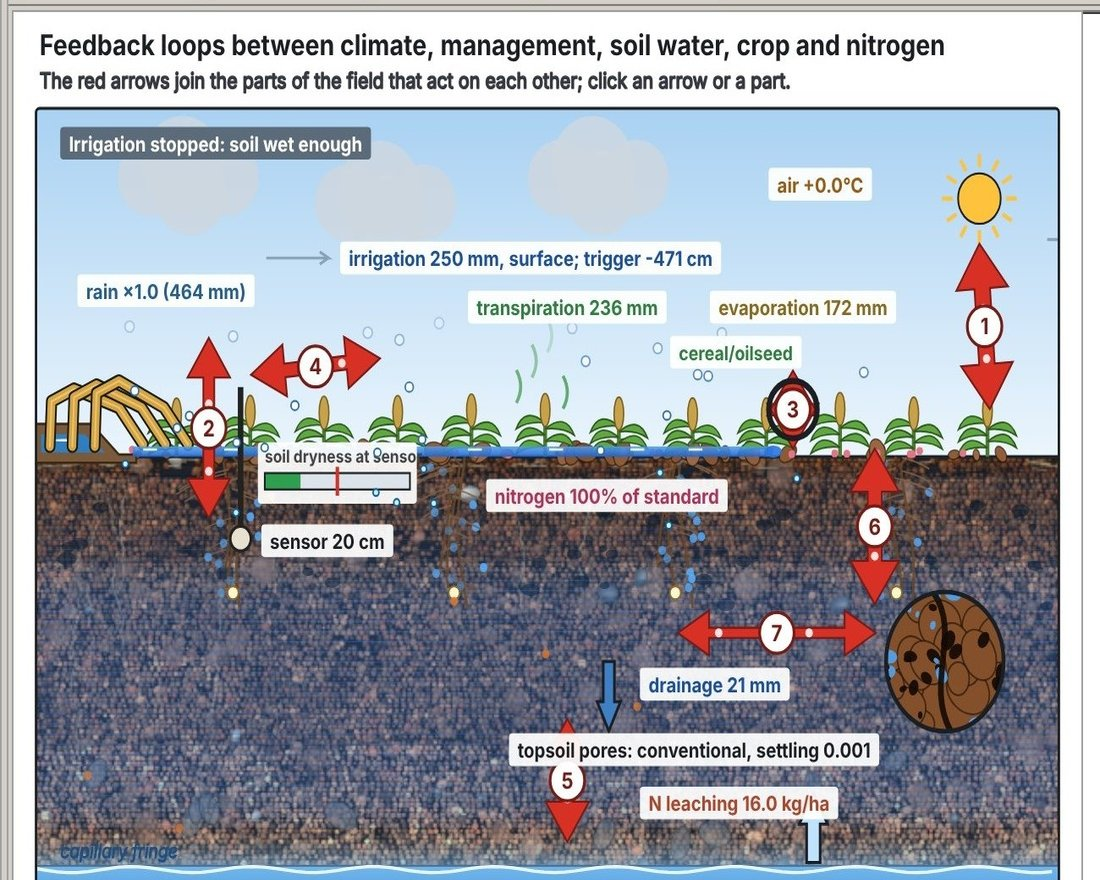
\includegraphics[width=0.67\paperwidth,height=0.37\paperheight]{fig/cv2.jpg}};
  \node[anchor=north west,inner sep=0] at ($(current page.north west)+(0,-0.825*\paperheight)$) {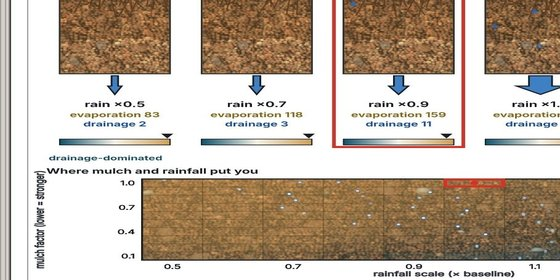
\includegraphics[width=0.33\paperwidth,height=0.108\paperheight]{fig/cv3.jpg}};
  \node[anchor=north,inner sep=0] at ($(current page.north)+(0,-0.825*\paperheight)$) {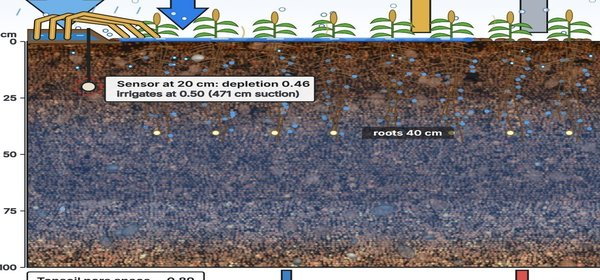
\includegraphics[width=0.34\paperwidth,height=0.108\paperheight]{fig/cv4.jpg}};
  \node[anchor=north east,inner sep=0] at ($(current page.north east)+(0,-0.825*\paperheight)$) {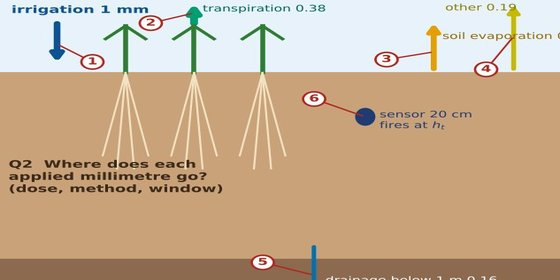
\includegraphics[width=0.33\paperwidth,height=0.108\paperheight]{fig/cv5.jpg}};
  \fill[white] ($(current page.south west)+(0,0.063*\paperheight)$) rectangle ($(current page.south west)+(0.34*\paperwidth,0.0*\paperheight)$);
  \node[anchor=west,text=khnavy,font=\sfb\itshape\fontsize{19}{20}\selectfont,inner sep=0] at ($(current page.south west)+(0.03*\paperwidth,0.032*\paperheight)$) {SWAFL};
  \shade[top color=khgold!70!white,bottom color=khgold!90!black,shading angle=90] (current page.south west) ++(0.34*\paperwidth,0) rectangle ($(current page.south east)+(0,0.063*\paperheight)$);
  \shade[top color=khgold!60!white,bottom color=khgold] ($(current page.south west)+(0,0.0*\paperheight)$) ++(0,0) rectangle ++(0,0);
\end{tikzpicture}
\cleardoublepage
\thispagestyle{empty}\vspace*{0pt}
{\sffamily\fontsize{11}{15}\selectfont Halilu, N.;\\ \textbf{Pore-Scale Dynamics}, a textbook of worked mathematics;\\ Soil Water, Atmosphere, Feedback and Layout (SWAFL) project, 2026;\\ Based on four studies, their Supplementary derivations, the SWAFL Desktop 1.1.0 manual and an open ensemble of 10,190 Daisy simulations (Zenodo, doi 10.5281/zenodo.23043626).\\ Licence: MIT.}
\clearpage
\pagestyle{front}
\begin{center}\vspace*{6mm}
\begin{tikzpicture}\node[font=\sfb\fontsize{26}{28}\selectfont,text=khred,inner sep=1pt] (c) {CONTENTS};\draw[khpurple,line width=3pt] ([yshift=3pt]c.west) -- ++(-2.2cm,0);\draw[khpurple,line width=3pt] ([yshift=3pt]c.east) -- ++(2.2cm,0);\end{tikzpicture}\end{center}
\vspace{3mm}
\newcounter{tocn}
\newcommand{\tocentry}[1]{%
 \par\noindent\begin{minipage}[t]{\textwidth}\vspace{4pt}%
  {\sfb\fontsize{11.5}{13.5}\selectfont\color{khblue}\makebox[1.2cm][l]{\csuse{chnum@#1}.}\parbox[t]{0.68\textwidth}{\csuse{chtitle@#1}}\hfill ...\csuse{chstart@#1}--\csuse{chend@#1}}\par\vspace{2pt}
  \hspace{1.2cm}\begin{minipage}[t]{0.50\textwidth}{\sffamily\fontsize{8.4}{10.4}\selectfont\color{khink}\setlength{\parindent}{0pt}\csuse{chtoc@#1}\par}\end{minipage}\hfill
  \begin{minipage}[t]{0.27\textwidth}\vspace{-1pt}\includegraphics[width=\linewidth,height=24mm,keepaspectratio]{\csuse{chimg@#1}}\end{minipage}%
 \end{minipage}\par}
\ifnum\totchap>0
\foreach \n in {1,...,\totchap}{\tocentry{\n}}
\fi
\cleardoublepage
\chapter*{How to use this book}
This book teaches, from first principles, the equations that sit behind the reach of a suction trigger, the fate of an irrigation millimetre, hydraulic memory and the audit of a water balance, and shows how each equation is derived from the outputs of the Daisy model. It follows the studies and the Supplementary derivations of the project, and every screenshot is taken from the SWAFL application.

\subhd{Structure.} Each chapter opens with a list of its features and a short statement of what you will be able to do. Then come the derivation, worked examples with numbers that you can reproduce with a pocket calculator or a few lines of code, boxes that say how a quantity is obtained from the Daisy outputs, and problems that are solved in full, step by step, directly after they are posed. No problem is left unsolved.

\subhd{Prerequisites.} Calculus, a first course in physics, and some familiarity with soil water. No knowledge of Daisy is assumed.

\subhd{Scope.} All findings concern a one-dimensional matrix-flow model; no field validation is claimed. Where a law is phenomenological and not derived from physics, the text says so.

\subhd{Status of this edition.} Part I presents the derivations. Part II works the mathematics of every SWAFL layer and of the Daisy workbench with computed examples.
\mainmatter
\pagestyle{fancy}
